\section{Motivație}

Volumul de date crește semnificativ de la an la an astfel până în 2020 se estimează că pentru fiecare persoană de pe planetă vor fi creați în fiecare secundă 1.7 MB de date, ceea ce înseamnă peste 13 milioane de GB creați în fiecare secundă în lume. În 2018 în fiecare minut se vizionau peste 97 de mii de ore de conținut pe Netlfix. Peste 4.3 milioane de videoclipuri erau vizionate pe Youtube. Pe Spotify se ascultau 750 de mii de melodii, iar Amazon pregătea peste o mie de colete \hyperlink{domo}{[1]}.

În România, Netflix pune la dispoziție 575 de filme și 208 seriale. În Regatul Unit sunt disponibile 2425 de filme și 542 de seriale, iar în Statele Unite ale Americii sunt disponibile 2942 de filme și 629 de seriale \hyperlink{finder}{[2]}. Amazon oferă cumpărătorilor o gamă cu un total de peste 119 milioane de produse, dintre care 44.2 milioane de cărți, 10.1 milioane de electronice sau 4.5 milioane de produse realizate manual \hyperlink{scrapehero}{[3]}.

Cu cât volumul de date pus la dispoziție de o platformă este mai mare cu atât este mai mare și necesitatea unui sistem de recomandare care să vină în ajutorul utilizatorului final pentru a explora mai ușor gama de produse oferită de respectiva platformă dar și în ajutorul deținătorului platformei care dorește să maximizeze, spre exemplu, vânzările sau vizionările. De asemnea, acel sistem de recomandare se vrea a fi îmbunătățit astfel încât să ofere fiecărui utilizator o experiență cât mai personalizată prin care să recomande, în cazul platformelor de streaming video, conținut relevant pentru a fi consumat de utilizatorul final, sau în cazul platformelor de ecommerce, produse pe care utilizatorul ar fi dispus să le cumpere.

În majoritatea cazurilor sistemele de recomandare se bazeaza pe metadatele utilizatorilor, precum: regiunea, vârsta, genul, ce alte produse a accesat sau cumpărat și metadatele produselor: categoria din care face parte, ratingul acestuia. La acestea se pot adăuga și alte informații precum: ce alte produse a apreciat un alt utilizator cu un profil asemanător.

\section{Obiective propuse}
În majoritatea cazurilor primul contact pe care îl avem cu un clip de pe Youtube, cu un film, serial de pe Netflix sau un produs de pe Amazon este contactul vizual cu imaginea de prezentare a acelui articol. 

Astfel, prezenta lucrare de disertație are drept obiectiv principal introducerea în sistemul de recomandare de informații vizuale extrase din imaginile de prezentare ale produselor, în cazul de față, posterele filmelor. Informațiile vizuale sunt reprezentate de clusterele create peste posterele asociate filmelor. Fiecare film are un set de postere dintre care se alege unul, iar acel poster are un cluster căruia îi aparține din intervalul $[1, N]$ unde $N$ este corelat cu numărul de genuri din baza de date pe care se execută optimizarea. $N$ poate fi ales și pe baza altor raționamente.

\begin{figure}[!htbp]
  \begin{subfigure}[b]{0.3\textwidth}
    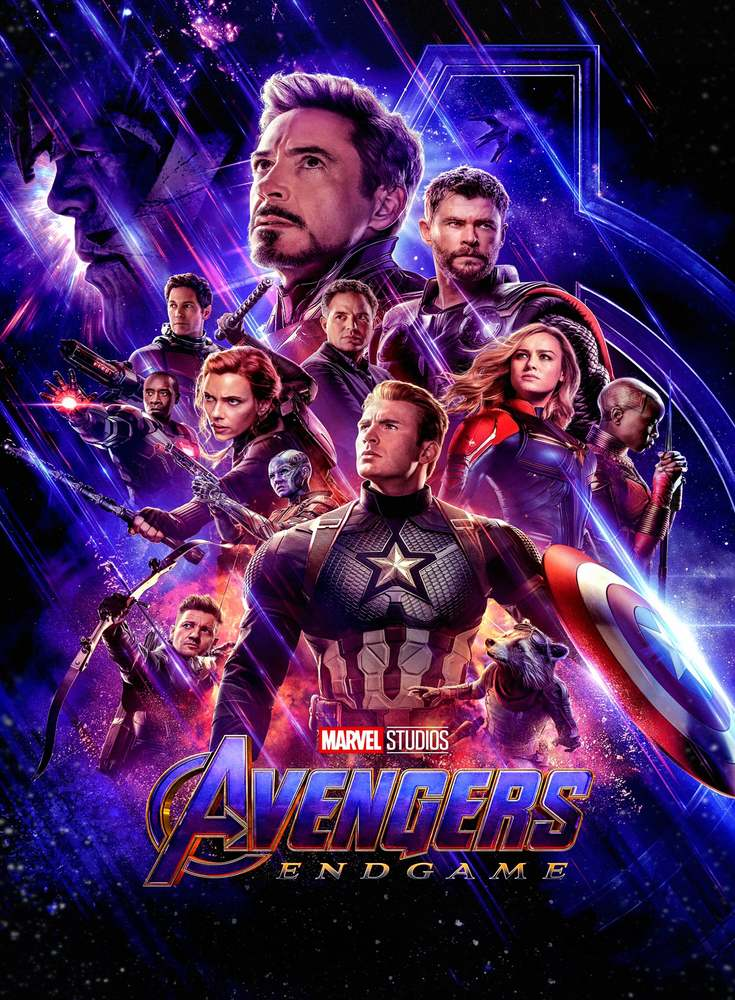
\includegraphics[width=\textwidth]{img_1_1}
  \end{subfigure}
  \hfill
  \begin{subfigure}[b]{0.3\textwidth}
    
\includegraphics[width=\textwidth]{img_1_2}
  \end{subfigure}
  \hfill
  \begin{subfigure}[b]{0.3\textwidth}
    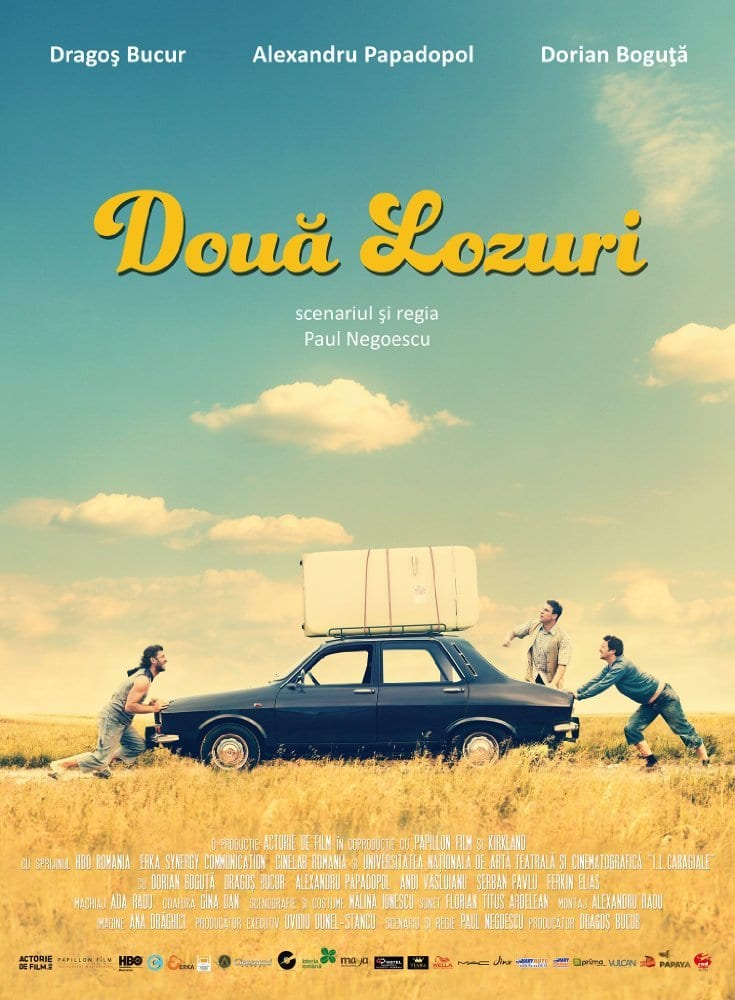
\includegraphics[width=\textwidth]{img_1_3}
  \end{subfigure}
  \caption[Exemple de postere]{\textit{Exemple de postere pentru diverse filme.}}
\end{figure}

Scopul final al acestei abordări fiind acela de a observa evoluția metricilor de evaluare, în cazul nostru, acurateațea și precizia@k, atunci când informația vizuală este introdusă într-un sistem de recomandare, fiind singura informație prezentă exceptând matricea de interacțiuni, dar și cum se comportă un sistem de recomandare când primește această informație împreună cu alte informații, spre exemplu genul unui film.

Acuratețea, în acest context, este definită ca fiind probabilitatea ca un exemplu pozitiv ales în mod aleator să fie clasat mai sus în recomandări decât un exemplu negativ ales în mod aleator. Precizia@k este definită de numărul de exemple pozitive aflate în primele $k$ recomandări.

\section{Structura lucrării}
Prezenta lucrare de disertație începe prin detalierea fundamentelor teoretice în capitolul II unde sunt prezentate teoriile ce stau la baza realizării acestei lucrări. În deputul capitolului definim noțiunile generale despre sistemele de recomandare, tipuri de sisteme de recomandare. Odată definite noțiunile de bază, prezentăm diversele strategii de recomandare, cu punctele lor tari și mai puțin tari, folosite în implementarea un astfel de sistem. Discuția despre sistemele de recomandare se încheie prin definirea funcțiilor de eroare folosite pentru optimizare într-un sistem. În continuare este prezentată metoda gradientului descendent, cu variante ale sale și cu algoritmi care optimizează această metodă. Tot în acest capitol sunt prezentate și noțiunile teoretice care stau la baza framework-ului LightFM folosit în implementarea soluției. Capitolul continuă cu prezentarea rețelelor neurale de la noțiunile generale până la rețelele folosite în implementare, VGG19, InceptionV3, ResNet și NASNet, pentru a transforma posterele filmelor în clustere. Acest capitol se termină cu prezentarea noțiunilor teoretice despre clustere și metrici de evaluare a lor.

Capitolul III este dedicat procesului de implementare al aplicației. Începe prin descrierea implementării modelului de recomandare și etapele de inițializare, antrenare și evaluare. Continuă prin descrierea procesului de clusterizare al posterelor, cum sunt transformate posterele filmelor în clustere. Este menționată și construcția bazei de date folosită în antrenarea și testarea modelului în sensul a ce tipuri de date conține și cum sunt reprezentare genurile filmelor și clusterele posterelor în această bază de date. În încheiere, este prezentat procesul de optimizare al parametrilor, optimizare care ajută modelul să identifice cei mai buni parametrii cu care poate avea cele mai bune rezultate în funcție de metadatele folosite în antrenare și testare.

Spre finalul lucrării, în capitolul IV, sunt descrise bazele de date folosite în cadrul prezentei aplicații. În cazul bazei de date cu postere este explicat procesul prin care a fost construită aceasta. Odată prezentate bazele de date, sunt prezentate și rezultatele obținute pe clusterizarea posterelor atât pe sanity check cât și rezultatele generale ale clusterelor pe toate posterele alese pentru filmele din baza de date. În finalul acestui capitol sunt prezentate rezultatele metricilor de precizie și acuratețe prin variația tipurilor de metadate folosite în model.

În încheierea lucrării sunt trase concluziile finale și sunt prezentate posibile viitoare
direcții de dezvoltare ale curentei aplicații.